\documentclass[11pt]{article}

\usepackage[margin=1in]{geometry}
\usepackage{amsmath,amssymb,amsthm,mathtools}
\usepackage{booktabs,tabularx,array}
\usepackage{graphicx}
\usepackage{caption}
\usepackage{float}
\usepackage{enumitem}
\usepackage{xcolor}
\usepackage[round]{natbib}
\usepackage{microtype}
\usepackage{titlesec}

% Compact run-in headings within each numbered subsection.
\titleformat{\subsubsection}[runin]
  {\normalfont\normalsize\bfseries}{\thesubsubsection}{0.6em}{}
\titlespacing*{\subsubsection}{0pt}{0.6\baselineskip}{0.6em}
\usepackage{hyperref}

\graphicspath{{../figures/}{figures/}}
\hypersetup{
  colorlinks=true,
  linkcolor=blue!50!black,
  citecolor=blue!50!black,
  urlcolor=blue!50!black
}

\setlength{\parindent}{0em}
\setlength{\parskip}{0.45em}
\setlength{\emergencystretch}{3em}
\setlist[itemize]{leftmargin=1.3em,itemsep=0.12em,topsep=0.12em}
\setlist[enumerate]{leftmargin=1.45em,itemsep=0.12em,topsep=0.12em}
\allowdisplaybreaks

\newtheorem{proposition}{Proposition}
\newtheorem{lemma}{Lemma}
\newtheorem{corollary}{Corollary}
\theoremstyle{definition}
\newtheorem{definition}{Definition}
\newtheorem{assumption}{Assumption}
\newtheorem{remark}{Remark}

\newcommand{\dd}{\mathrm d}
\newcommand{\E}{\mathbb E}
\newcommand{\1}{\mathbf 1}

\title{Intergenerational Housing Misallocation and Fertility}
\author{Tommaso De Santo}
\date{}

\begin{document}

\maketitle
\begin{abstract}
\end{abstract}

\pagebreak
\section{Introduction}
\label{sec:introduction}

% Author text.

% October 5, 2026 build: same preamble and structure as JMP_DS_mock.tex,
% with the new empirical subsection and the new model section. Agent draft.
\newcommand{\mocktodo}[1]{\textcolor{red}{[TODO: #1]}}
% ============================================================================
% NEW MATERIAL, October 6, 2026 (agent draft; not in JMP_DS_draft).
% Motivating-evidence section for the oct05 build. It reorganizes, without
% editing them, sections/02_empirical_evidence.tex (housing around the first
% birth, Sept 24), the fertility facts of 02b, and the "Who holds the large
% homes" subsection of the Oct 4 sandbox paper
% (tmp/jmp_paper_sandbox_20261004/paper/sections/02_empirical_evidence.tex,
% reviewed there against primary sources). Calibration data and targets now
% live in Section 4. Register: Boar, Gorea and Midrigan, Section 2.
% ============================================================================
\providecommand{\mocktodo}[1]{\textcolor{red}{[TODO: #1]}}

\section{Motivating Evidence}
\label{sec:empirical-evidence}

This section documents four facts that shape the model. First, children
arrive early in adult life, and earliest in lower-income families. Second,
large homes are mostly owned. Third, most large owner-occupied homes are held
by older households without children at home, while young families hold few.
Fourth, households enlarge their dwelling and move into ownership within a few
years of the first birth, and then move less. Together these facts describe
how a young family obtains space for children: it needs a larger home at the
start of adult life, when its savings are smallest, and the large homes are
mostly sold rather than rented and mostly held by an older generation. None
of the facts isolates an exogenous change in fertility, and I do not use them
to argue that housing costs lower fertility. Appendix~\ref{app:empirical-data}
describes the data.

\subsection{Children arrive early}

First births are concentrated in the mid twenties. In the 2003--2006 natality
records the mean age of mothers at first birth is 26.0 years, and a woman aged
25 in the 2004 and 2006 Current Population Survey (CPS) has had 0.81 children.
% [DATA] NCHS 2003-06, 25.976; CPS June 2004/06 women aged 25, 0.810 (capped at 3).
Early childbearing is concentrated in lower-income families.
Table~\ref{tab:emp-fertility-income} groups women in the 2024 CPS fertility
supplement into thirds of family income. Among women aged 24 to 26, those in
the bottom third have had 0.60 children and those in the top third 0.23. By
ages 40 to 44 the gradient has nearly disappeared: 1.78 children in the bottom
third and 1.73 in the top. Lower-income women do not have many more children
over their lives; they have them earlier, at the ages at which households
have the least wealth. The fact describes who has children early, not how
income affects fertility: young women who live with their parents report
their parents' income, and a birth itself lowers a mother's earnings.
Restricting the sample to women who head a household or are married to its
head makes the young gradient steeper, not flatter.

\begin{table}[t]
\centering
\caption{Children ever born by family income (CPS, 2024)}
\label{tab:emp-fertility-income}
\begin{tabular}{lcccc}
\toprule
 & Bottom third & Middle third & Top third & Top minus bottom \\
\midrule
Women aged 24--26 & 0.596 & 0.448 & 0.226 & $-0.369$ \ $(0.052)$ \\
Women aged 40--44 & 1.784 & 1.702 & 1.733 & $-0.051$ \ $(0.050)$ \\
\bottomrule
\end{tabular}
\par\smallskip
\begin{minipage}{0.92\linewidth}
\footnotesize\textit{Notes:} June 2024 CPS Fertility Supplement. Mean
children ever born, capped at three, weighted by the person weight. Thirds
are equal-weight groups of family money income in the previous twelve months.
Approximate standard errors in parentheses, clustered by household. 1,673
women aged 24--26 and 3,278 aged 40--44.
% [DATA] output/model/credit_mechanism_20261004/measurement/tables.json.
\end{minipage}
\end{table}

\subsection{Large homes are owned}

Figure~\ref{fig:tenure-by-size} divides the homes of each size in the 2023
American Housing Survey (AHS) by tenure. Of the homes with four or more
bedrooms, 87 percent are owner-occupied and 9 percent are rented; of the homes
with at most one bedroom, 13 percent are owner-occupied and 74 percent are
rented. Measured in rooms, the unit used in the rest of the paper, 43.0
percent of owner-occupied homes have seven or more rooms, against 7.5 percent
of rented homes. The gap persists among families: in households with children,
owners occupy 6.8 rooms on average and renters 5.2. Nearly half of renter households
with children, 48.7 percent, live in homes with at most two bedrooms,
against 7.4 percent of owner households with children.
% [DATA] AHS 2023 ahs_children_space_mismatch.csv (code/data/ahs_supply_snapshot/
% output_ahs_family_unit_menu_national/). These shares describe the
homes households occupy, not the homes offered for rent. They show that, in
the existing stock, a family that wants a large dwelling typically buys one.
% [DATA] AHS 2023 national PUF; code/data/ahs_supply_snapshot/ (sandbox
% FIGURES.md maps the figure to its source).

\begin{figure}[t]
\centering
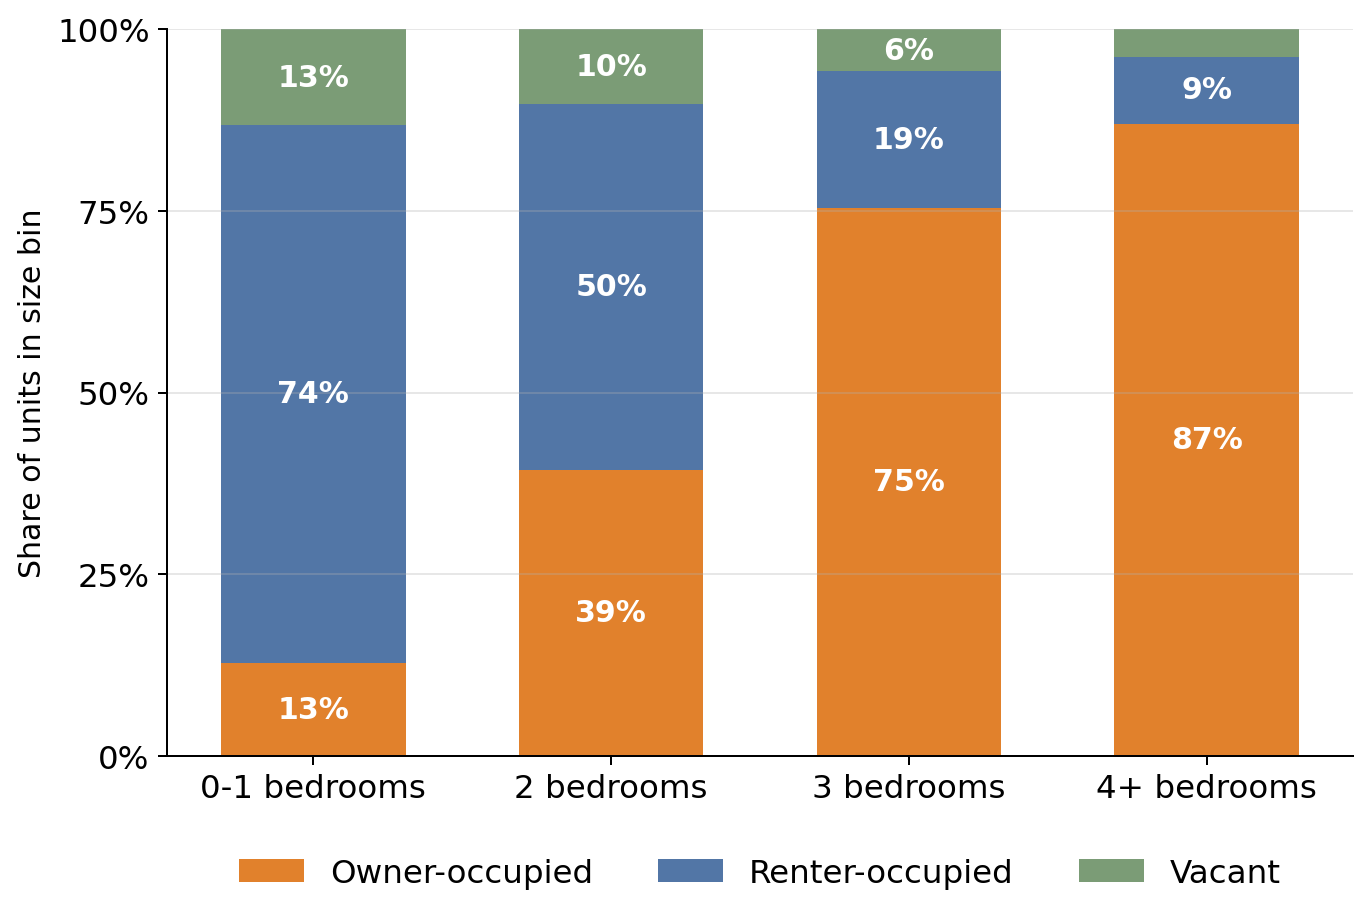
\includegraphics[width=0.62\linewidth]{ahs_tenure_share_within_size}
\caption{Tenure of the housing stock by number of bedrooms (AHS 2023)}
\label{fig:tenure-by-size}
\par\smallskip
\begin{minipage}{0.92\linewidth}
\footnotesize\textit{Notes:} Each bar divides the housing units with the
stated number of bedrooms into owner-occupied units, units rented for cash,
and vacant units. Units occupied without payment of cash rent and units whose
occupants have a usual residence elsewhere are excluded. Weighted by the
housing-unit weight. Source: American Housing Survey 2023, national
public-use file.
\end{minipage}
\end{figure}

\subsection{Who holds the large homes}

Most large owner-occupied homes are held by households without children at
home, and the largest group among them is old. Figure~\ref{fig:large-homes}
divides the owner-occupied homes with six or more rooms in 42 large
metropolitan areas in the 2023 American Community Survey (ACS) among six groups
of households, defined by the age of the householder and by whether a child of
the householder younger than 18 lives in the home. Households aged 60 to 85
without children at home hold 40.0 percent of these homes, and households
aged 40 to 59 without children at home another 21.8 percent. Households aged
22 to 39 with children hold 10.6 percent. Across all ages, 68.3 percent of the
large owner-occupied homes house no child of the householder, close to the
72.9 percent of all households in these areas without a child at home. What
the figure shows is therefore where the large homes sit by age, not that
childless households hold more than their share. I call the concentration of
large owner-occupied homes among older households the intergenerational
allocation of housing. The figure does not show that older households would
sell at some price, or that young families would have more children if they
held these homes.
% [DATA] ACS 2023 one-year, 42 metros, householders 22-85, 289,109 households;
% numbers as in the Oct 4 sandbox paper (reviewed there).
\mocktodo{name the builder of the large-homes figure in the data appendix
(not found in code/ by the Oct 4 sandbox review); the sandbox calls this
"intergenerational misallocation", which the title uses; choose the term.}

\begin{figure}[t]
\centering
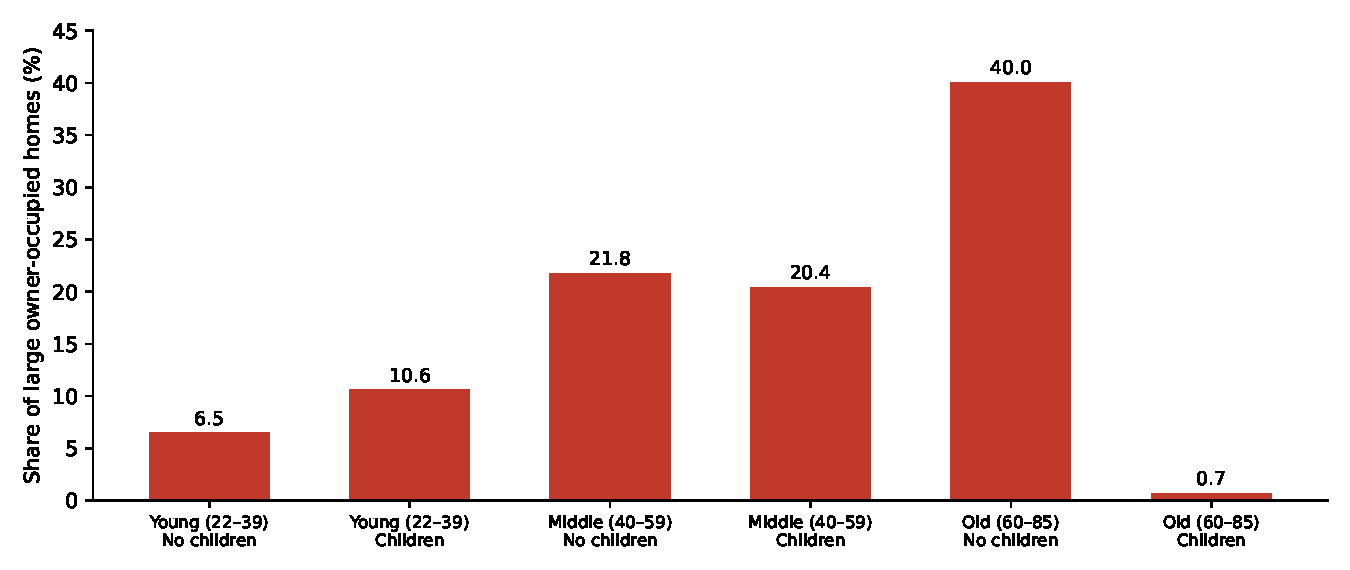
\includegraphics[width=0.9\linewidth]{large_homes_by_age_children_acs2023}
\caption{Who holds the large owner-occupied homes (ACS 2023)}
\label{fig:large-homes}
\par\smallskip
\begin{minipage}{0.92\linewidth}
\footnotesize\textit{Notes:} Each bar is the share of owner-occupied homes
with six or more rooms held by households in the group; the six shares sum to
100 percent. Groups are defined by the age of the householder and by whether
an own child of the householder younger than 18 lives in the household.
Householders aged 22 to 85 in 42 large metropolitan areas, weighted by the
household weight; 289,109 households.
\end{minipage}
\end{figure}

\subsection{Housing around the first birth}

The Panel Study of Income Dynamics (PSID) follows the same families from 1968
to 2019. I date each woman's first birth from her full history of biological
children and estimate event studies of her household's housing around it,
comparing first-time mothers with women who never have children, with the
estimator of Sun and Abraham (2021) and person and year
fixed effects. The reference window is two to three years before the birth,
so that moves made while expecting a child count as responses. The sample
keeps one woman per household and year who is its reference person or spouse.
% [DATA] mock 02_empirical_evidence.tex and data_appendix.tex; 63,338
% person-years, 3,655 first-time mothers, 1,654 childless women.

Households add about one room within four years of the first birth.
Figure~\ref{fig:emp-rooms-path} reports the path. The dwelling is 0.41 rooms
larger than in the reference window in the year of the birth, 0.82 rooms one
to two years later, and 1.03 rooms (standard error 0.07) three to four years
after it, on a base of 4.7 rooms. Fixing household position before the birth,
which removes a pre-trend that reflects who heads a household, the increase at
three to four years is 1.47 rooms (0.05). The added space comes with a move
into ownership, after which families move less (Figure~\ref{fig:emp-tenure-moves}).
The ownership rate is 11 percentage points higher in the birth window and 16
points higher three to four years later, on a base of 41 percent. The
probability of having moved since the previous interview falls by 16 to 21
points after the birth and stays lower for a decade, and among those who do
move, the share moving for more space doubles, from 12 to about 25 percent.
The ACS shows the same pattern at a point in time: among household heads aged
30 to 55, those whose oldest child is under four are 12.8 percentage points
more likely to own than heads without children.
% [DATA] ACS 2005-06 recent-parent gap 0.12761 (same as Section 4 target).

\begin{figure}[t]
\centering
\includegraphics[width=0.88\linewidth]{first_birth_rooms_psid}
\caption{Rooms around the first birth (PSID)}
\label{fig:emp-rooms-path}
\par\smallskip
\begin{minipage}{0.92\linewidth}
\footnotesize\textit{Notes:} Interaction-weighted event-study estimates in
two-year windows of event time, with 95 percent confidence intervals from
standard errors clustered by person. One woman per household-year who is the
reference person or spouse; 63,338 person-years, 3,655 first-time parents and
1,654 childless women. The hollow marker is the omitted reference window,
years $-3$ and $-2$. Mean rooms in the reference window: 4.70.
\end{minipage}
\end{figure}

\begin{figure}[t]
\centering
\includegraphics[width=0.92\linewidth]{first_birth_tenure_moves_psid}
\caption{Ownership and moving around the first birth (PSID)}
\label{fig:emp-tenure-moves}
\par\smallskip
\begin{minipage}{0.92\linewidth}
\footnotesize\textit{Notes:} Same sample, estimator and reference window as
Figure~\ref{fig:emp-rooms-path}. ``Moved for more space'' equals one if the
household moved since the previous interview and gave more space as the first
reason. Means in the reference window: ownership 0.41, moved 0.58.
\end{minipage}
\end{figure}

\subsection{Implications for the model}

These facts motivate the main features of the model. Because children arrive
early and need space, fertility and housing are chosen jointly over the life
cycle, with a minimum of space for parents. Because large homes are mostly
owned, the size of dwelling a family can occupy depends on its tenure; the
model limits the size of rental units, so a family that wants a large home
must buy it, with a down payment it accumulates by saving. Because the large
homes sit with older households, the price of space for young families depends
on the whole age distribution of households; the model is an
overlapping-generations economy in which the house price clears one market
shared by all ages.

% ============================================================================
% NEW MATERIAL, October 5, 2026 (agent draft for Tommaso; not in JMP_DS_draft).
% A complete Model section written to the model as implemented at the base
% point promoted Oct 6 (output/model/production/2007: Estate A + net-estate
% floor, balanced property-tax rebate, PSID levels entry; loss 15.07,
% provisional, native postcheck passed). First drafted on chain 11,
% engine code/model/experiments/birth_count_choice/model/engine/.
% It does not replace sections/03_model.tex, which is left unchanged; the
% October 5 build (JMP_DS_mock_oct05.tex) inputs this file instead.
% Where the code and the author's stated intent differ, the text follows the
% intent and a TODO marks the difference. Calibrated values are placeholders
% until the Estate A refit; fixed inputs carry their source in a comment.
% ============================================================================
\providecommand{\mocktodo}[1]{\textcolor{red}{[TODO: #1]}}

\section{Model}
\label{sec:model-oct05}

Motivated by these observations, I build a life-cycle model in which the same
households choose when to have children, how much housing to occupy, and
whether to rent or own it. Households live in an overlapping-generations
economy, face persistent earnings risk, and save in a single bond. Children
raise the household's needs for consumption and, above all, for space. Space
can be rented or bought. Renting and owning the same dwelling cost the same per
period, but the largest dwellings are available only to owners, owners enjoy
their home somewhat more, selling a home is costly, and buying one requires a
down payment that must be accumulated by saving. House prices and rents are
determined in equilibrium by an upward-sloping supply of housing. The
government runs a pay-as-you-go pension system and taxes property.

\subsection{The economy}

Time is discrete and a period lasts four years.
% [MODEL INPUT] period_years 4.0 (bundle).
I describe the households, their preferences, the earnings process, housing,
the financial market and the government in turn.

\subsubsection*{Demographics.}
A household enters the economy at age 18 and lives at most through age 85, for
$J$ periods indexed by $j$. It works until retirement at age 66 and then
receives a pension. From retirement on, it survives from one period to the
next with probability $s_j<1$; before retirement $s_j=1$.
% [MODEL INPUT] ages 18,22,...,82 (17 cells), J_R = cell 12 (age 66),
% survival 0.9391, 0.9185, 0.8850, 0.8300 for cells 12-15, certain death after
% age 82. Source of the survival schedule not documented in the repo.
\mocktodo{name the source of the survival probabilities (not documented in the
repository; ask Tommaso).}
Each household is one decision unit; I do not model the formation or
dissolution of couples.

Let $n$ denote the number of children ever born to the household and $m$ the
number currently living at home. Births are possible at ages 18 to 45, at most
one per period. Each child at home leaves independently with probability
$\lambda$ per period, so that a child stays on average $1/\lambda$ periods;
departure lowers $m$ but not $n$. I keep track of $n$ up to three, with the
last state standing for three or more.
% [MODEL INPUT] fertile cells ages 18-42 (decision at the start of each
% four-year period, so births up to age 45); lambda = 2/9 per four-year
% period, mean stay 18 years; no newborn exemption; top state n = 3 = "3+".

\subsubsection*{Preferences.}
A household values consumption $c$, housing services $s$, and children at
home. Its flow utility is
\begin{equation}
 u(c,s;m)
 =\frac{1}{1-\sigma}\left(\frac{c^{\alpha}s^{1-\alpha}}{e(m)}\right)^{1-\sigma}
 +\psi\, m^{1-\gamma}.
 \label{eq:m5-utility}
\end{equation}
The first term is utility from the consumption--housing composite per
equivalent adult. The equivalence scale
\begin{equation}
 e(m)=\left(\frac{2+\omega m}{2}\right)^{\nu}
 \label{eq:m5-escale}
\end{equation}
measures how many adult equivalents the household contains, so that the same
spending buys less utility per person in a larger family. The second term is
the direct benefit of children at home, with $\psi>0$ its level and
$\gamma\in[0,1)$ the rate at which the benefit of an additional child
declines.
% [MODEL INPUT] e(m) code: ((2+0.7 m)/2)**0.7, multiplied into utility as
% e**(sigma-1); omega = nu = 0.7, m top-coded at 3. Code form
% e^(sigma-1) * x^(1-sigma)/(1-sigma) equals (x/e)^(1-sigma)/(1-sigma).
\mocktodo{cite the source of the equivalence scale ($\omega=\nu=0.7$); the
September deck cites Scholz et al.\ (2006), not checked against the paper.}

Children need room. A household with children at home obtains services only
from the space in excess of a minimum $h_P$:
\begin{equation}
 s=
 \begin{cases}
 h^R-h_P\,\mathbf 1\{m\geq1\}, & \text{renter of } h^R \text{ rooms},\\[2pt]
 \chi\bigl(h-h_P\,\mathbf 1\{m\geq1\}\bigr), & \text{owner of } h \text{ rooms},
 \end{cases}
 \qquad \chi\geq1 .
 \label{eq:m5-services}
\end{equation}
The parent floor $h_P$ is the space a family needs before additional rooms
add to its welfare. The floor is measured in rooms, and the ownership
premium $\chi$ applies only to the rooms above it. It does not depend on the number of children, so it is
the first child that creates the need for space. The parameter $\chi$
captures the additional services an owner obtains from a dwelling of a given
size, for example from the ability to adapt it.
% [MODEL INPUT/CODE] hbar_child_rooms = 0; owner composite is chi*(h - h_P)
% (kernels.py 858-871), not chi*h - h_P as on the September slides.
% Settled: the floor does not grow with children (open object, fine for now).
% Author decision Oct 6: keep the code form chi*(h - h_P); an experiment with
% chi*h - h_P may follow.
Together, \eqref{eq:m5-utility} and \eqref{eq:m5-services} define what a
child costs. At given prices, a first child raises the spending needed to
reach a given utility in two ways: through the equivalence scale, which
scales up all spending, and through the floor, which must be paid at the
rental price of space before any housing yields services.

\subsubsection*{Fertility.}
At the start of each fertile period, a household chooses whether to try for a
child. An attempt succeeds with probability $\pi_j$, which declines with age.
A first birth carries a one-time utility cost $\xi$ of becoming a parent. The
decision is subject to type-I extreme-value taste shocks with scale $\kappa_1$
when the household is childless and $\kappa_C$ when it already has children.
After the outcome of the attempt is known, the household chooses its housing
and saving for the period.
% [MODEL INPUT] pi_j = 1 - 0.02 exp(0.134 (age - 18)), zero from 45;
% fecundity constants unfitted (open item). Fertility logit scales
% kappa_fert (n = 0) and kappa_fert_continuation (n >= 1).
Housing can therefore adjust to a birth within the same period, which matches
the timing of the room response in Section~\ref{sec:empirical-evidence}.

\subsubsection*{Earnings.}
Before retirement, a household of age $j$ earns
\begin{equation}
 y_j(z)=(1-\tau^w)\,w\,\varepsilon_j\,z ,
 \label{eq:m5-earnings}
\end{equation}
where $w$ is the wage, normalized to one, $\varepsilon_j$ a deterministic
age profile, $\tau^w$ the payroll tax, and $z$ an idiosyncratic productivity
state. Productivity follows a first-order autoregressive process in logs,
\begin{equation}
 \log z'=(1-\rho)\mu_z+\rho\log z+\eta',\qquad \eta'\sim N(0,\sigma_\eta^2),
 \label{eq:m5-ar1}
\end{equation}
where $\mu_z$ normalizes mean productivity to one. Earnings risk is the
only source of income uncertainty. Retirees receive a
pension $\varpi$ that is the same for all retirees.
% [MODEL INPUT] rho = 0.735, sigma_eta = 0.484 per four-year period (annual
% 0.926, 0.270), sigma_z = 0.713, mu_z = -0.252 (E[z] = 1). Method of moments,
% PSID gross labor earnings EARNINDRRC, annual waves 1984-1997, non-overlapping
% four-year block means residualized on age and year, rho = 0.3735/0.5085;
% bootstrap rho [0.692, 0.769]. Traced by the utility thread, Oct 6.
% Earlier note: rho = 0.7346, sigma_eta = 0.4838 at four-year frequency,
% estimated by method of moments on PSID four-year log-earnings
% autocovariances (single_process_external_estimate.json); nine-state
% discretization; age profile from breakpoints 22/26/34/46/58. Pension flat
% (retirement_income_z_scale = 0), level balanced endogenously.
\mocktodo{name the data source of the age profile $\varepsilon_j$ (not
documented in the files read).}

\subsubsection*{Housing.}
Housing is measured in rooms and trades at price $P$ per room. Owners choose
among dwellings of $h\in\mathcal H=\{2,4,6,8,10\}$ rooms. Renters choose any
size up to $\bar h^R$ rooms, so the largest dwellings can only be owned, as in
the American Housing Survey facts of Section~\ref{sec:empirical-evidence}.
Owners pay depreciation $\delta$ and property tax $\tau^H$ on the value of
their home each period. Selling a home costs a fraction $\varsigma$ of its value;
buying costs nothing beyond the price.
% [MODEL INPUT] H = {2,4,6,8,10}; rental cap 6 rooms (retained provisional);
% delta = 1.416% a year, tau_H = 1.060% a year (adopted national inputs);
% selling cost 6%.
A household's tenure and dwelling choice is subject to type-I extreme-value
taste shocks with scale $\kappa_H$, one for each option: renting, keeping the
current home, or buying each size in $\mathcal H$.

Competitive landlords own the rental stock. A landlord buys a room at $P_t$,
pays depreciation and property tax, rents it out at $r_t$, and sells it at
$P_{t+1}$. Landlords finance themselves at the household bond return $R$, so
zero profits require
\begin{equation}
 r_t=(R+\delta+\tau^H)P_t-P_{t+1},
 \qquad\text{and in a steady state}\qquad
 r=(R-1+\delta+\tau^H)P .
 \label{eq:m5-rent}
\end{equation}
Rent per room equals the owner's user cost.
Because the rent equals the user cost and households and landlords borrow and
save at the same rate, a room costs the same per period whether it is rented or
owned. Tenure matters for the cost of a family through four features only: the
size limit on rentals $\bar h^R$, the ownership premium $\chi$, the cost of
selling $\varsigma$, and the down payment described next.

Housing is supplied by a competitive construction sector with a constant
elasticity with respect to the rental price,
\begin{equation}
 H^s_t=H_0\left(\frac{r_t}{\bar r}\right)^{\zeta},
 \label{eq:m5-supply}
\end{equation}
where $H_0$ sets the scale of the stock, $\bar r$ is a normalizing rent and
$\zeta$ is the supply elasticity.
% [MODEL INPUT] xi_supply = 0.63 (pinned; the 1.75 eta_supply field is unread);
% r_bar = 0.16; H0 = 6.2996 derived at N = 1. Whether supply should respond to
% gross- or net-of-tax rent is an open item in CALIBRATION_STATUS.md.

\subsubsection*{Saving and mortgages.}
Households save in a one-period bond with gross return $R$, fixed in the world
market. Let $b$ denote the bond position a household carries into a period;
$b<0$ is mortgage debt. Borrowing must be secured by a home: renters cannot
borrow, and an owner of $h$ rooms can borrow up to a fraction $\phi$ of the
home's value,
\begin{equation}
 b'\geq-\phi\,P h .
 \label{eq:m5-ltv}
\end{equation}
A buyer must therefore end the period of purchase holding equity of at least
$(1-\phi)Ph$, the down payment. Since $b'$ is the outcome of the household's
consumption--saving choice, the down payment is accumulated through saving;
there is no separate rule for how it is financed. The constraint applies to
any new borrowing. An owner whose debt exceeds $\phi Ph$ after a fall in the
price is not forced to repay, but cannot borrow more. Mortgages carry no
amortization schedule and no limit on payments relative to income.
% [CODE] native_due_stayer_credit: stayer floor min(b, -phi P h);
% mortgage_amortization 0; no PTI. phi = 0.80 (fixed, non-negotiable).
% The engine also screens purchases on R b + y; that screen is implied by
% (eq:m5-ltv) at the end of the period and is not written here (see the
% October 1 assessment in memory).

\subsubsection*{Budget constraints.}
Transactions in housing take place after interest accrues on the bond carried
into the period. Let $S=(1-\varsigma)P h_{-}$ denote the proceeds from selling the
home a household enters the period with, if any, and $Q=Ph$ the price of a home
it buys. A household that rents $h^R$ rooms faces
\begin{equation}
 c+r\,h^R+b'=Rb+y+T+S,
 \qquad b'\geq0,
 \label{eq:m5-bc-rent}
\end{equation}
and a household that owns $h$ rooms at the end of the period faces
\begin{equation}
 c+(\delta+\tau^H)P h+b'=Rb+y+T+S-Q,
 \qquad b'\geq-\phi Ph,
 \label{eq:m5-bc-own}
\end{equation}
with $S=0$ for a household that did not own and $S=Q=0$ for an owner who
keeps its home. Here $y$ is earnings or the pension and $T$ a lump-sum
transfer from the government. The sale proceeds and the purchase price are not
compounded: a household that sells and buys within a period carries only the
difference between them into next period's interest.
% [CODE] post-interest timing, author-adopted: b' = R b + S - Q + y - c - K
% (kernels.py 301/316/331, 379/394/409; household.py 306). The September
% slides still show the original timing b' = R(b + S - Q) + y - c - K.

\subsubsection*{Estates.}
A household that dies leaves its net estate, the bond plus the value of its
home net of the selling cost, $W=b'+(1-\varsigma)Ph'$. It values the estate
according to
\begin{equation}
 v(W)=\theta_0\,\frac{(\theta_1+W)^{1-\sigma}-\theta_1^{1-\sigma}}{1-\sigma},
 \label{eq:m5-bequest}
\end{equation}
where $\theta_0$ governs the strength of the bequest motive and $\theta_1$ the
extent to which bequests are a luxury. Estates are not received by other
households in the model; entrants' wealth is drawn from the data instead, as
described below.
% [CODE] Estate A: bequest_utility_vec(b + (1-psi) P h), normalized,
% theta_n = 0, estate tax 0, no recipient; settled as intended for now.
% Net-estate floor b' >= -(1-psi) P h' where death is possible; slack at
% phi = 0.8, so not stated.

\subsubsection*{Government.}
The government runs two programs, each with a balanced budget. The pension
system pays every retiree the same pension $\varpi$, financed by the payroll
tax $\tau^w$ on earnings. The property tax raises $\tau^H$ times the value of
the entire housing stock, owned and rented, and its revenue is returned to
all households as an equal lump-sum transfer $T$.
% [MODEL, base_2007, Oct 6 refit 15.07] balanced rebate on inside every solve
% (tmp/rebate_entry_impl_20261006; output/model/production/2007). Chains 11
% and 13 had no rebate; that discrepancy is resolved at the new base.
% [MODEL INPUT] pension_mode balanced_stationary; tau_w = 0.0803 from the CPS
% ASEC pension/earnings ratio 0.2294; pension 0.918 per period (derived).
% The September slides cite a 17.9% payroll tax; the code uses 0.0803.

\subsubsection*{Entry.}
Households enter at age 18 as childless renters. Each entrant draws its
productivity from the stationary distribution of $z$. Its wealth comes from the
distribution of net worth among childless renters aged 18 to 24 who head their
household in the PSID, 1984 to 2019, with negative net worth set to zero.
Dollar amounts are converted to model units with one common scale, chosen so
that mean income in this sample equals mean earnings of entrants in the model,
and observations are assigned to productivity states by income rank, so that
the poorest entrants in the data become the least productive entrants in the
model. The number of entrants in each period equals the number of children
born sixteen to twenty years earlier divided by $2.1$, so that the population
is constant when each household has $2.1$ children on average.
% [MODEL, base_2007] entry law levels_rank (author decision Oct 5-6):
% closure_root/.../model/entry_wealth.py; N = 1,835 family-years, 29.6% with
% negative net worth (censored at zero). Earnings in the scale exclude all
% transfers. Replaces the chain-11 five-bin rescaled rule.
% [CODE] adult_entry.py: entry = adjusted births / 2.1, half entering 16
% years after birth and half 20; adjusted births count a birth into the
% top state as 3.602 children (provisional). The 0.5 entrant_conversion_factor
% is read only by an outside-flow valve that is off at chain 11.

\subsection{The household's problem}
\label{sec:m5-household}

The state of a household at the start of a period is its age $j$,
productivity $z$, bond position $b$, number of children ever born $n$ and at
home $m$, and housing $h_{-}$, which is either a home it owns or zero for a
renter. A period has three stages. The household first chooses whether to try
for a child, then chooses tenure and dwelling, and finally chooses consumption
and saving. Children leave home and productivity is drawn between periods.

\subsubsection*{Saving.}
Consider a household that has decided to own $h$ rooms and enters the saving
stage with cash on hand $x=Rb+y_j(z)+T+S-Q$. Its value is
\begin{multline}
 V^O_j(x,z,n,m,h)=\max_{c,\,b'}\;u\bigl(c,\chi(h-h_P\mathbf 1\{m\geq1\});m\bigr)\\
 +\beta\,\mathbb E\Bigl[s_j\,\mathcal W_{j+1}(b',z',n,m',h)+(1-s_j)\,v\bigl(b'+(1-\varsigma)Ph\bigr)\Bigr]
 \label{eq:m5-vown}
\end{multline}
subject to \eqref{eq:m5-bc-own}. The expectation is over next period's
productivity $z'$ and the number of children $m'$ still at home. The renter's
value $V^R_j(x,z,n,m)$ is defined in the same way, with the choice of $h^R\leq
\bar h^R$, the renter's services, and the constraint \eqref{eq:m5-bc-rent}.
Because the composite in \eqref{eq:m5-utility} is Cobb--Douglas, a renter not
at the size limit spends a share $1-\alpha$ of its outlay net of the floor on
rooms above $h_P$.

\subsubsection*{Tenure and dwelling.}
Let $o$ index the options available to a household entering the period with
housing $h_{-}$: renting, keeping its home if it owns one, or buying a dwelling
of each size in $\mathcal H$. Each option implies its own cash on hand and its
own saving-stage value, $V_o$. An option is available only if it leaves room
for a saving choice that satisfies the borrowing constraint. With the
extreme-value shocks, the value of entering this stage is
\begin{equation}
 \mathcal H_j(b,z,n,m,h_{-})=\kappa_H\log\sum_{o}\exp\bigl(V_o/\kappa_H\bigr),
 \label{eq:m5-tenure}
\end{equation}
and the probability of choosing option $o$ is
$\exp(V_o/\kappa_H)/\sum_{o'}\exp(V_{o'}/\kappa_H)$.

\subsubsection*{Fertility.}
At the start of a fertile period, a household with $n<3$ compares not trying,
which leaves it at $\mathcal H_j(b,z,n,m,h_-)$, with trying, which yields
\[
 U^1_j=\pi_j\bigl[\mathcal H_j(b,z,n+1,m+1,h_-)-\xi\,\mathbf 1\{n=0\}\bigr]
 +(1-\pi_j)\,\mathcal H_j(b,z,n,m,h_-).
\]
With scale $\kappa=\kappa_1$ if $n=0$ and $\kappa=\kappa_C$ otherwise, the
value at the start of the period is
\begin{equation}
 \mathcal W_j(b,z,n,m,h_-)=\kappa\log\Bigl[\exp\bigl(\mathcal H_j(b,z,n,m,h_-)/\kappa\bigr)
 +\exp\bigl(U^1_j/\kappa\bigr)\Bigr].
 \label{eq:m5-fertility}
\end{equation}
Outside the fertile ages, or with $n=3$, $\mathcal W_j=\mathcal H_j$.

\subsection{Equilibrium}

I study stationary equilibria, in which prices and the distribution of
households over states are constant, and transitions between them.

\begin{definition}
A stationary equilibrium consists of a house price $P$ and rent $r$; a pension
$\varpi$ and payroll tax $\tau^w$; a transfer $T$; decision rules for
fertility, tenure, dwelling size, consumption and saving; and a distribution
$\mu$ of households over states, such that
\begin{enumerate}
\item the decision rules solve the household problem of Section~\ref{sec:m5-household} given
prices, taxes and transfers;
\item the rent satisfies the landlord's zero-profit condition
\eqref{eq:m5-rent};
\item the housing market clears: the rooms occupied by owners and renters
equal the supply \eqref{eq:m5-supply},
\[
 \int\Bigl[\mathbf 1\{\text{own}\}\,h+\mathbf 1\{\text{rent}\}\,h^R\Bigr]\dd\mu
 =H_0\left(\frac{r}{\bar r}\right)^{\zeta};
\]
\item the pension system balances, $\tau^w w\int\varepsilon_j z\,
\mathbf 1\{j<J_R\}\dd\mu=\varpi\int\mathbf 1\{j\geq J_R\}\dd\mu$, and the
transfer returns property-tax revenue, $T\int\dd\mu=\tau^H P\int\bigl[
\mathbf 1\{\text{own}\}\,h+\mathbf 1\{\text{rent}\}\,h^R\bigr]\dd\mu$;
\item $\mu$ is the stationary distribution implied by the decision rules, the
earnings process, survival, the departure of children, and entry, with the
mass of entrants equal to past births divided by $2.1$.
\end{enumerate}
\end{definition}

Two features of the equilibrium are worth stating. First, the price of
housing is what links fertility to housing supply: more births raise the
demand for rooms by families, which raises $P$ and $r$ and with them the cost
of the space a child requires. Second, because the population is constant
only if each household has $2.1$ children on average, the scale of housing
supply $H_0$ and the level of fertility are tied together in a stationary
equilibrium. In the quantification I normalize the population to one and
choose $H_0$ so that the market clears at the price consistent with a constant
population.%
\footnote{Equivalently, the price is the one at which the stationary
population reproduces itself, and $H_0$ is the supply scale that makes that
price clear the housing market. A counterfactual holds $H_0$ fixed and lets
the population adjust.}
\mocktodo{check this closure paragraph against Tommaso's intended
wording; the code solves the price from the renewal condition and derives
$H_0$ (production/README.md lines 18--19).}

% ----------------------------------------------------------------------------
% ----------------------------------------------------------------------------
% Parameter values for Section 4 must be read from the base point:
%   python3 code/model/tools/read_results.py fit base_2007
%   output/model/production/2007/parameters_estate_a.csv
% (Oct 6 refit, Mac chain 7, case 0129_nm, loss 15.0712, provisional;
% e.g. beta 0.9397, psi 0.157, chi 1.081, h_P 2.585, H0 6.312). Not typeset.
% ----------------------------------------------------------------------------

\paragraph{Open items for the author (mock only).}
\mocktodo{(1) Whether the income
gradient of Table~\ref{tab:emp-fertility-income} is an untargeted evaluation
fact, and whether to recompute it on the 2004 and 2006 CPS. (2) The wording of
the equilibrium closure (price from the renewal condition, $H_0$ derived).
(3) Sources for the survival probabilities, the age profile $\varepsilon_j$
and the equivalence scale.}

% ============================================================================
% NEW MATERIAL, October 6, 2026 (agent draft; not in JMP_DS_draft).
% Adapted from sections/04_quantification.tex (Sept 23, organized after
% Boar, Gorea and Midrigan), which is left unchanged. Numbers are the base
% point promoted Oct 6: output/model/production/2007 (Oct 6 refit, Mac chain 7,
% case 0129_nm; one-birth Estate A + net-estate floor, balanced property-tax
% rebate, PSID levels entry; loss 15.0712 on the 14-row contract; provisional,
% fresh native postcheck passed). Read with
%   python3 code/model/tools/read_results.py fit base_2007
% Conversions traced in tmp/rebate_entry_impl_20261006/closure_root/code/model
% (inputs.py:76 beta; e5f_social_security.py:41 income; parameters.py:1237
% child departure; tools/e5f_initial_fertility_observer.py age windows;
% engine/distribution.py:2435 bequest annualization).
% ============================================================================
\providecommand{\mocktodo}[1]{\textcolor{red}{[TODO: #1]}}

\section{Quantification}
\label{sec:quant-oct06}

I calibrate a stationary economy representing 2007, before the subsequent
decline in fertility. I use observations from the surrounding years to
discipline fertility, housing, and household wealth. Fertility moments come
from the 2004 and 2006 CPS and the 2003--2006 natality records, housing moments
from the 2005--2006 ACS, the 2007 AHS and the PSID, and wealth from the 2005
and 2007 PSID and the 2007 SCF. This steady state is the starting point for the
historical transition.

I organize the parameters into two groups. The first is set outside the
estimation, from external evidence or direct measurement. The second is
estimated by matching model moments to their empirical counterparts. I first
describe the data behind the targets. Before describing either group of
parameters, I then explain how annual data map into the model's
four-year period, because almost every parameter and moment passes through
that mapping.

\subsection{Data}
\label{sec:quant-data}

The targets combine five data sets, each chosen for the object it measures
best. Table~\ref{tab:quant-fit-oct06} lists every moment with its source.

\paragraph{Fertility.} The June Fertility Supplement of the CPS records the
number of children ever born to each woman. I pool the 2004 and 2006
supplements and measure childlessness and the share of mothers with exactly
one child among women aged 40 to 44, and the mean number of children ever born
among women aged 25. Children ever born are capped at three, the largest
number the model distinguishes. The timing of first births comes from the
NCHS natality files, which record every birth with the mother's age and the
birth order; I pool first births in 2003 to 2006.

\paragraph{Housing.} Mean rooms come from the 2007 AHS, for household heads
aged 18 to 85, without top-coding. Ownership among household heads aged 30 to
55 and the ownership gap between recent parents, whose oldest child is under
four, and heads without children come from the 2005--2006 ACS.
\mocktodo{state the dwelling-structure restriction used in both ACS ownership
moments (UNITSSTR codes 3--10 in the builder) and whether the model imposes it.}
The room response to the first birth is the PSID event-study estimate of
Section~\ref{sec:empirical-evidence} in the sample that fixes household
position before the birth: 1.465 rooms three to four years after the birth
(standard error 0.050). I use this sample rather than the household sample of
Figure~\ref{fig:emp-rooms-path}, which gives 1.03, because the model follows
the same households before and after the birth.

\paragraph{Wealth.} Aggregate net worth relative to aggregate annual gross
labor earnings comes from the 2005 and 2007 PSID: net worth of all household
heads aged 18 to 85, excluding business and farm equity and other real
estate, over gross labor earnings of heads aged 18 to 65. The bequest flow is
the annual flow of estates directed to children relative to aggregate net
worth in the 2007 Survey of Consumer Finances.
% [DATA] builders: CPS code/data/cps_fertility/; NCHS
% code/data/nchs_natality_timing/build_first_birth_timing.R; AHS
% code/data/ahs_supply_snapshot/build_ahs_2007_room_target.py; ACS
% code/empirical/housing/build_initial_housing_profile_diagnostic.py; PSID rooms
% code/data/psid_followup_mar2026/sa_rooms_first_birth_v2.do (A2h); SCF
% code/data/scf/build_bequest_flow_2007.py. Target fingerprint c7a3d185...

\subsection{From annual data to four-year periods}
\label{sec:quant-period}

A model period lasts four years. The unit of account is mean annual gross
labor earnings of working-age households, so a model value of one corresponds
to \$82,882 in the 2005 and 2007 PSID (2022 dollars).
% [DATA] metadata.json normalizers: psid_annual_gross_labor_age18_65 82881.95;
% model_annual_gross_labor_before_retirement 1.0522.
The mapping follows three rules.

\paragraph{Stocks are measured in annual units; flows are four years long.}
Wealth, house prices and the bequest shifter $\theta_1$ are stocks and are not
rescaled. Income, consumption, rent and every other flow accrue over the whole
period, so a flow in the model is four times its annual counterpart. For
example, an entrant at age 18 with average productivity earns
$4\times(1-0.080)\times0.721=2.65$ per period after the payroll tax, which is
0.72 times mean annual gross earnings.
% [MODEL] e5f_social_security.py:41: income = period_years*(1-tax)*wage*profile;
% first profile cell 0.72055. Annual gross recovered as income/4/(1-tau).
A moment that relates a stock to a flow is computed against the annual flow,
as in the data: the wealth target divides net worth by annual gross earnings,
and the bequest target divides the estate flow over a period by four before
dividing it by aggregate wealth.

\paragraph{Rates compound; hazards come from durations.}
Interest, discounting and depreciation compound over the four years. The gross
return is $R=1.02^4=1.082$, the period discount factor is $\beta=\beta_{\text{ann}}^4$,
and the period depreciation rate is $1-(1-\delta_{\text{ann}})^4$. With
$\beta_{\text{ann}}=0.940$, the period discount factor is $0.780$. The property
tax is the exception: it is a tax on value levied each year, and I set the
period rate to four times the annual rate.%
\footnote{Compounding instead would give a period rate of 4.17 rather than
4.24 percent of value.}
\mocktodo{confirm the linear property-tax convention; the code calls it
explicit and not interchangeable with compounding.}
Probabilities of events are period probabilities. Children leave home after
18 years on average, which I implement as a constant departure probability of
$\lambda=1/4.5=2/9$ per period for each child. Survival probabilities are
four-year probabilities between successive age cells. The probability $\pi_j$
that an attempt to have a child succeeds is the probability of a conception
within four years at that age.
% [MODEL] parameters.py:68,76,1237 (A_m = 18, stage duration 4.5 periods);
% fecundity pi = 1 - 0.02 exp(0.134 (age-18)); docs/model/
% fecundity_schedule_note_20260720.tex fits within-four-year conception
% probabilities (91/84/64% at 30/35/40).
\mocktodo{cite the source of the four-year conception probabilities named in
docs/model/fecundity\_schedule\_note\_20260720.tex, and the life table behind
the survival probabilities.}
The earnings process is estimated directly at the four-year frequency rather
than converted from an annual process. I take non-overlapping four-year means
of household gross labor earnings in the annual PSID waves of 1984--1997,
remove age and year effects, and estimate $\rho=\gamma_1/\gamma_0=0.735$ from
the first two autocovariances of their logarithm. The implied annual
persistence is $0.735^{1/4}=0.926$.
% [DATA] single_process_external_estimate.json: gamma0 0.5085, gamma1 0.3735,
% sigma_eta 0.484, bootstrap rho [0.692, 0.769]; EARNINDRRC.

\paragraph{Age-specific moments use the overlap of data ages with model cells.}
A model household of age $j$ occupies the four-year cell $[a_j,a_j+4)$. A data
statistic for an age window weights each cell by the fraction of the cell that
falls in the window. Within a cell, a household's number of children is
interpolated linearly between its value at the start and at the end of the
cell, which is exact if births are spread uniformly over the four years. Two
examples show how this works. Women aged 40 to 44 overlap the cell
$[38,42)$ for half its length and the cell $[42,46)$ for three-quarters of its
length, and in each cell the stock of children is read at the midpoint of the
overlap. Children ever born at age 25 are read from the cell $[22,26)$,
seven-eighths of the way from its start to its end. For the mean age at first
birth, I date a first birth in the model at the midpoint of its cell (20, 24,
\ldots, 44) and group the natality data into the same four-year cells, so that
both sides use the same representative ages.
% [MODEL] tools/e5f_initial_fertility_observer.py:154 (midpoints), 163-182
% (40-44 overlap weights 0.5 and 0.75; post shares 0.75 and 0.375),
% 185-218 (age 25: post share (25.5-22)/4 = 0.875).

The room response to the first birth is the one moment for which the period
length bounds how closely the model can mimic the data. In the model, I
compare households that have a first birth with otherwise identical
households that do not, one period, or four years, after the birth. The data
compare years three and four after the birth with years two and three before
it. The model's contrast is therefore a four-year response with no
pre-period, while the data's spans about six years.
\mocktodo{decide whether to state the six-year versus four-year difference this
plainly; the measurement review (docs/model/e5f\_target\_measurement\_review\_20260927.md)
calls the model observer an approximation, not the same estimator.}

\subsection{Parameters set outside the estimation}

Table~\ref{tab:quant-assigned-oct06} summarizes the parameters assigned
outside the estimation.

\paragraph{Demographics and preferences.}
Households enter at age 18, retire at 66, and live at most through age 85.
Survival is certain before retirement. Children remain at home for 18 years
on average. Births are possible through age 45, with the success probability
of an attempt falling from 0.98 at 18 to 0.50 at 42. I set risk aversion to
$\sigma=2$ and use the power equivalence scale with child weight $\omega=0.7$
and exponent $\nu=0.7$. The consumption weight $\alpha=0.733$ is the
expenditure share of nonhousing consumption among childless renters in the
2019--2023 CEX. A birth into the state of three or more children counts as
3.60 children when computing completed fertility: the mean number of
children, capped at five, among women aged 40 to 44 with three or more in the
2024 CPS.
% [MODEL INPUT] tfr_top_bin_weight 3.602359 (provisional; author review).

\paragraph{Housing finance and transaction costs.}
The annual real return on the bond is 2 percent, and selling a home costs 6
percent of its value \citep{greaneyDynamicUrbanEconomics2025}. Annual
depreciation is 1.416 percent and the annual property tax is 1.060 percent of
value. Mortgage debt cannot exceed $\phi=0.80$ of the value of the home, so an
owner must hold at least 20 percent equity at the end of the period in which
it buys. There is no payment-to-income limit.
\mocktodo{name the sources of the depreciation and property-tax rates (recorded
as "adopted national inputs").}

\paragraph{Income and pensions.}
The deterministic age profile of earnings is normalized to average one over
working ages. Productivity follows the four-year process described above, with
$\rho=0.735$ and innovation standard deviation $0.484$, approximated with nine
states. Entrants draw productivity from its stationary distribution. Every
retiree receives the same pension. I set the payroll tax so that the pension
equals 22.9 percent of mean annual gross earnings, the ratio of pension
income to gross earnings in the CPS ASEC; the stationary pension budget then
implies a payroll tax of 8.0 percent.
% [MODEL INPUT] pension_period 0.91778 = 4 x 0.22945; tau_pay 0.080281.
\mocktodo{confirm the pension/earnings ratio's CPS ASEC year and definition.}

\paragraph{Housing products and supply.}
Owners choose among homes of $\{2,4,6,8,10\}$ rooms. Renters choose any size
up to $\bar h^R=6$ rooms. The supply of housing has an elasticity of
$\zeta=0.63$ with respect to rent. The supply scale $H_0$ is not a free
parameter: given the other parameters, it is the value at which the housing
market clears at the price consistent with a constant population.
% [MODEL INPUT] xi_supply 0.63 ("fixed provisional external mapping");
% H0 derived = 6.3117 at N0 = 1.
\mocktodo{cite the source of $\zeta=0.63$ (the September deck cites
Baum-Snow and Han (2024); check before citing).}

\paragraph{Entry wealth and bequests.}
Entrants' wealth follows the PSID rule of Section~\ref{sec:model-oct05}:
net worth of childless renters aged 18 to 24, censored at zero and assigned to
productivity states by income rank. Under Estate A the bequest motive does not
depend on the number of children. I fix the bequest shifter $\theta_1$ at 1
percent of median annual gross earnings, $\theta_1=0.008$.

\begin{table}[H]
\centering
\caption{Parameters set outside the estimation}
\label{tab:quant-assigned-oct06}
\small
\begin{tabularx}{\textwidth}{@{}X l X@{}}
\toprule
Parameter & Value & Evidence or restriction \\
\midrule
Model period & 4 years & Model timing \\
Entry, retirement, maximum ages & 18, 66, 85 & Life-cycle specification \\
Child departure per period $\lambda$ & $2/9$ & Mean stay of 18 years \\
Success of a birth attempt $\pi_j$ & 0.98 (18) to 0.50 (42) & Four-year conception probabilities \\
Risk aversion $\sigma$ & 2 & Maintained \\
Equivalence scale $(\omega,\nu)$ & $(0.7,0.7)$ & Maintained power scale \\
Consumption weight $\alpha$ & 0.733 & CEX 2019--2023, childless renters \\
Annual real return & 2\% & \citet{greaneyDynamicUrbanEconomics2025} \\
Annual depreciation; property tax & 1.416\%; 1.060\% & National inputs \\
Financed share $\phi$ & 0.80 & 20\% equity requirement \\
Selling cost $\varsigma$ & 6\% & \citet{greaneyDynamicUrbanEconomics2025} \\
Pension / mean annual earnings & 0.229 & CPS ASEC; implies payroll tax 8.0\% \\
Persistence $\rho$ (four-year) & 0.735 & PSID 1984--1997 \\
Innovation SD $\sigma_\eta$ (four-year) & 0.484 & PSID 1984--1997 \\
Owner house sizes & 2, 4, 6, 8, 10 rooms & \\
Largest rental unit $\bar h^R$ & 6 rooms & \\
Housing-supply elasticity $\zeta$ & 0.63 & \\
Entry wealth & PSID levels & Childless renters 18--24, censored at zero \\
Bequest shifter $\theta_1$ & 0.008 & 1\% of median annual earnings \\
\bottomrule
\end{tabularx}
\end{table}

\subsection{Internally estimated parameters}

I estimate ten parameters jointly to match ten moments, listed in
Table~\ref{tab:quant-fit-oct06}. In addition, the stationary population
requires mean completed fertility of 2.1, which the house price delivers in
equilibrium. Although all parameters are identified jointly, I organize the
discussion by economic block and describe which moments are most informative
about each.

\paragraph{Saving.}
The annual discount factor governs how much households carry across ages.
Aggregate net worth relative to aggregate annual gross earnings is the most
informative moment. The target is a ratio of totals, not an average of
household ratios.

\paragraph{Housing demand and tenure.}
The room response around the first birth is the most informative moment for
the parent floor $h_P$: the larger the floor, the more rooms a household must
add when its first child arrives. Mean rooms disciplines housing demand more
broadly. The ownership rate and the ownership gap between recent parents and
childless households are most informative about the ownership premium $\chi$
and the dispersion $\kappa_H$ of tenure taste shocks.

\paragraph{Fertility.}
Childlessness is most informative about the first-birth cost $\xi$. The mean
age at first birth and the number of children by age 25 discipline the timing
of first births, and with it the dispersion $\kappa_1$ of first-birth taste
shocks. The share of mothers with exactly one child is most informative about
the dispersion $\kappa_C$ for later births and the curvature $\gamma$ of the
child benefit. The level of the child benefit $\psi$ moves all fertility
moments together.

\paragraph{Bequests.}
With $\theta_1$ fixed, the bequest flow relative to aggregate wealth is most
informative about $\theta_0$.

\begin{table}[H]
\centering
\caption{Internally estimated parameters}
\label{tab:quant-parameters-oct06}
\small
\begin{tabularx}{\textwidth}{@{}l X r X@{}}
\toprule
Parameter & Interpretation & Value & Most informative moments \\
\midrule
$\beta_{\text{ann}}$ & Annual discount factor & 0.940 & Wealth / earnings \\
$\xi$ & First-birth utility cost & 0.309 & Childlessness \\
$\kappa_1$ & First-birth taste dispersion & 0.121 & First-birth age; children by 25 \\
$\kappa_C$ & Later-birth taste dispersion & 0.356 & Exactly one child \\
$\psi$ & Child benefit, level & 0.157 & All fertility moments \\
$\gamma$ & Child benefit, curvature & 0.098 & Exactly one child \\
$h_P$ & Parent floor (rooms) & 2.585 & First-birth room response; mean rooms \\
$\chi$ & Ownership premium & 1.081 & Ownership; recent-parent gap \\
$\kappa_H$ & Tenure taste dispersion & 0.018 & Ownership; recent-parent gap \\
$\theta_0$ & Bequest strength & 0.212 & Bequests / wealth \\
\addlinespace
$H_0$ & Supply scale (derived) & 6.312 & Market clearing at constant population \\
\bottomrule
\end{tabularx}
\par\smallskip
\begin{minipage}{0.95\linewidth}
\footnotesize\textit{Notes:} Search bounds: $\beta_{\text{ann}}\in[0.93,0.99]$,
$h_P\in[0.1,2.6]$, $\kappa_1,\kappa_C\in[0.02,50]$.
\mocktodo{$h_P$ is within 0.015 of its upper bound and the search flags
$\kappa_1$ and $\kappa_C$ as near their bounds; decide how to report this.
$\beta_{\text{ann}}=0.9397$ is below the 0.94 floor recorded as an external
restriction in July; confirm which restriction applies.}
% [MODEL] output/model/production/2007/parameters_estate_a.csv.
\end{minipage}
\end{table}

\subsection{Target moments and fit}

Table~\ref{tab:quant-fit-oct06} reports the targets and the model's values.
The model matches childlessness, the share with exactly one child, the timing
of first births, ownership, the recent-parent ownership gap and the wealth and
bequest ratios closely. It misses two moments. Households in the model have
0.55 children by age 25 against 0.81 in the data, so first births start too
late even though their mean age is matched. And the model's family adds 1.26
rooms around the first birth against 1.47 in the data, with the floor $h_P$
near its upper bound.

\begin{table}[t]
\centering
\caption{Targets and model moments, 2007 steady state}
\label{tab:quant-fit-oct06}
\small
\begin{tabularx}{\textwidth}{@{}X l r r@{}}
\toprule
Moment & Data & Target & Model \\
\midrule
\multicolumn{4}{@{}l}{\emph{Fertility}}\\
Childlessness, women 40--44 (\%) & CPS 2004, 2006 & 19.83 & 20.20 \\
Exactly one child among mothers 40--44 (\%) & CPS 2004, 2006 & 21.37 & 21.76 \\
Mean age at first birth (years) & NCHS 2003--2006 & 25.98 & 25.99 \\
Children ever born at age 25 & CPS 2004, 2006 & 0.810 & 0.551 \\
First births at age 30+ (\%)$^{\dagger}$ & NCHS 2003--2006 & 24.93 & 23.88 \\
\addlinespace
\multicolumn{4}{@{}l}{\emph{Housing}}\\
Mean rooms, heads 18--85 & AHS 2007 & 5.729 & 5.816 \\
Ownership, heads 30--55 (\%) & ACS 2005--2006 & 67.63 & 66.68 \\
Recent-parent ownership gap (pp) & ACS 2005--2006 & 12.76 & 12.72 \\
Rooms added around the first birth & PSID 1968--2019 & 1.465 & 1.260 \\
Rooms, 3+ minus 1--2 children$^{\dagger}$ & ACS 2005--2006 & 0.385 & 0.295 \\
\addlinespace
\multicolumn{4}{@{}l}{\emph{Wealth}}\\
Net worth / annual gross earnings & PSID 2005, 2007 & 4.458 & 4.576 \\
Bequests / wealth (\%) & SCF 2007 & 0.729 & 0.702 \\
p90/p50 wealth-to-income, ages 76--84$^{\dagger}$ & PSID 2003--2005 & 3.516 & 3.307 \\
\addlinespace
Mean completed fertility (equilibrium condition) & --- & 2.10 & 2.10 \\
\bottomrule
\end{tabularx}
\par\smallskip
\begin{minipage}{0.95\linewidth}
\footnotesize\textit{Notes:} $^{\dagger}$ Not targeted. Samples and definitions in
Section~\ref{sec:quant-data}.
\end{minipage}
\end{table}
% Full fit (base_2007, loss 15.0712): moment | target | model | gap | weight | loss
% cps_childlessness .198279 .202033 +.003755 35532.3 0.5009
% cps_exactly_one .213655 .217574 +.003919 26952.8 0.4139
% nchs_mean_age 25.97626 25.98889 +.012624 139.828 0.0223
% nchs_share30 .249278 .238803 -.010475 0 0 (validation)
% wealth_earnings 4.458387 4.576325 +.117938 7.5951 0.1056
% bequest_wealth .0072910 .0070194 -.000272 5165289.3 0.3811
% old_dispersion 3.515935 3.306923 -.209012 0 0 (validation)
% mean_rooms 5.729434 5.816323 +.086888 128.021 0.9665
% ownership_30_55 .676260 .666805 -.009455 2339.36 0.2091
% first_birth_rooms 1.465 1.259836 -.205164 137.565 5.7904
% family_rooms .385100 .295259 -.089841 0 0 (validation)
% recent_parent_ownership .127608 .127185 -.000423 27055.8 0.0048
% early_fertility .809528 .551139 -.258389 100 6.6765
% initial_normalization 2.1 2.1000001 (normalization, unscored)

% ============================================================================
% NEW MATERIAL, October 6, 2026 (agent draft; not in JMP_DS_draft).
% Results section skeleton. Every number is from the base point
% output/model/production/2007 (Oct 6 refit, loss 15.07, provisional) unless a
% comment says otherwise:
%   untargeted moments: output/model/production/2007/plotted_long.csv
%   price and credit arms: output/model/jmp_draft_deck_20261005/
%     refit_best_15p07_credit/results.csv (fixed price fp_*, stationary GE ge_*)
% Results that exist only at chain 11, chain 13 or the Sept 14 point are
% NOT typeset; they are listed in comments as the rerun queue.
% ============================================================================
\providecommand{\mocktodo}[1]{\textcolor{red}{[TODO: #1]}}

\section{Results}
\label{sec:results}

This section uses the calibrated economy to ask how housing costs and access
to credit shape fertility. I first evaluate the model on moments it was not
asked to match. I then raise the price of housing and, separately, relax the
down-payment requirement, and trace each change to births, ownership and the
size of homes. Finally, I describe the historical exercise, in which the
economy moves from 2007 to 2023.

\subsection{Moments not targeted}

The model reproduces the distribution of first births by age, although only
the mean age was targeted: in the model 34.6 percent of first births occur
before age 22 and 11.9 percent at ages 30 to 33, against 34.2 and 14.3 percent
in the data. It misses in three places, each informative about the mechanism.
% [MODEL] plotted_long.csv first_birth_age, cells 18,22,...; data NCHS.

First, young households own too much. At age 24, 42.9 percent of households
in the model own their home, against 23.5 percent in the data; by age 40 the
two agree, at 67.2 and 66.5 percent. The model matches ownership at ages 30
to 55 by having households buy earlier than they do in the data.
\mocktodo{name the data source of the ownership-by-age profile in the
assessment packet (model\_data\_assessment.pdf).}

Second, the first child raises space too much. Households with one child
occupy 7.3 rooms in the model and 5.9 in the data, against 5.0 and 5.1
without children. This is the other side of the miss on the first-birth room
response in Table~\ref{tab:quant-fit-oct06}: the model adds too few rooms
around the birth itself but ends up with too many once the child is there.
\mocktodo{these two statements are hard to reconcile without the event-time
paths; check the rooms-by-children observer (cross-section, all ages) against
the event-study observer before keeping the sentence.}

Third, and most important, the model gets the income gradient of fertility
wrong. Among households aged 24 to 26, those in the bottom third of income
have 0.15 children in the model and 0.61 in the data, and those in the top
third 0.94 and 0.23. By ages 40 to 44 the model's gradient is still positive,
1.50 against 2.31, while the data's is slightly negative. In the model, the
cost of the parent floor is a large share of income for the poorest
households, so they postpone or forgo children; in the data they have them
earliest. Section~\ref{sec:results-price} shows why this matters for the
response of births to housing costs.
% [MODEL] plotted_long.csv income_24_26 (Model .149/.554/.943; Data
% .608/.453/.226), income_40_44 (Model 1.498/1.969/2.311; Data
% 2.013/1.891/1.851). The data columns differ from Table 1 (0.596/.../1.784):
% different grouping (assessment packet vs measurement/tables.json).
\mocktodo{use one definition of the CPS income thirds in Table~\ref{tab:emp-fertility-income}
and here; the assessment packet and the Section 2 table differ by up to 0.28
children at 40--44.}

\subsection{Housing costs and births}
\label{sec:results-price}

The cost of a child in the model has two parts. The equivalence scale raises
the spending needed to keep consumption per person constant, and the parent
floor requires $h_P$ rooms before housing yields any services. The second part
is large. At the calibrated price, a room rents for 0.141 per period, so the
floor costs $0.141\times2.585=0.363$ per period, or 9.1 percent of mean annual
earnings each year. For a household entering at 18 with average productivity
it is 12.6 percent of its gross earnings.
% [MODEL] r = user_cost_rate 0.18028 x P 0.77952 = 0.14053 per room per
% period; h_P 2.58534; annual 0.0908; entrant annual gross 0.72055.

I raise the house price and the rent by 10 percent and hold all other prices
and policies fixed. Births fall by 4.9 percent. Ownership at ages 18 to 29
falls by 2.8 percentage points, and young households occupy 6.6 percent fewer
rooms. Table~\ref{tab:results-experiments} reports the full set of
responses.
% [MODEL] fp_price110: births -4.8828%, own 18-29 -2.7936 pp, rooms 18-29
% -6.5557%, mean rooms -5.9773%.
\mocktodo{split the price effect into an income effect and the cost of the
floor at the base point (rerun the Shapley split; it exists only at chain 11,
where the floor accounts for 60 percent and income for 45 percent).}
\mocktodo{add the stationary general-equilibrium version of the price
experiment; only the fixed-price arm exists at the base point.}

\subsection{Credit and births}
\label{sec:results-credit}

Because rent equals the user cost of an owner and households and landlords
face the same interest rate, a room costs the same per period whether it is
rented or owned. The down-payment requirement therefore governs when a
household can buy, not what its space costs over the life cycle. I raise the
financed share $\phi$ from 0.80 to 0.95, holding prices fixed. Ownership at
ages 18 to 29 rises by 25 percentage points, from 43 to 68 percent, and
births fall by 1.4 percent. With $\phi=1$, ownership rises by 29 points and
births fall by 1.3 percent.
% [MODEL] fp_phi095: births -1.4400%, own 18-29 +25.10 pp (0.4335 -> 0.6845);
% fp_phi100: births -1.3480%, own 18-29 +28.82 pp.

The fall in births comes from the homes that newly eligible buyers choose.
Among childless households aged 18 to 37, the share that owns a two-room home
rises from 6.7 to 42.2 percent. Two rooms are below the parent floor, so a
household in such a home must move before it can have a child, and moving
costs 6 percent of the home's value out of little equity.
% [MODEL] refit_best_15p07_credit/README.md starter-home check: renter /
% 2-room owner / larger owner 74.1/6.7/19.3 -> 28.4/42.2/29.4 at phi .95.
\mocktodo{decompose the credit effect at the base point into the change in
decisions at a given state and the change in the distribution of states
(exists only at chains 11 and 13; at chain 11 the distribution term dominates).}

In a stationary equilibrium, completed fertility must equal replacement, so a
change in credit cannot change births per household in the long run; it
changes the price at which the population replaces itself, and the size of the
population. With $\phi=0.95$, the stationary price is 2.9 percent lower and
the number of households 3.0 percent lower.
% [MODEL] ge_phi095: price -2.936%, population_scale 0.97053, births
% per household -0.08% (closure); ge_phi100: price -1.978%, scale 0.98365.
\mocktodo{check the sign and wording of the population result with Tommaso
before keeping it; it is a stationary comparison, not a transition.}

\begin{table}[t]
\centering
\caption{Responses to housing costs and credit, 2007 steady state}
\label{tab:results-experiments}
\small
\begin{tabular}{lrrrr}
\toprule
 & Births (\%) & Ownership 18--29 (pp) & Rooms 18--29 (\%) & Price (\%) \\
\midrule
\emph{Fixed prices} & & & & \\
House price and rent $+10\%$ & $-4.88$ & $-2.79$ & $-6.56$ & $+10.0$ \\
Financed share $0.80\to0.95$ & $-1.44$ & $+25.10$ & $-0.84$ & 0 \\
Financed share $0.80\to1.00$ & $-1.35$ & $+28.82$ & $-0.71$ & 0 \\
\addlinespace
\emph{Stationary equilibrium} & & & & \\
Financed share $0.80\to0.95$ & $-0.08$ & $+27.03$ & $+1.32$ & $-2.94$ \\
Financed share $0.80\to1.00$ & $-0.10$ & $+28.92$ & $+0.97$ & $-1.98$ \\
\bottomrule
\end{tabular}
\par\smallskip
\begin{minipage}{0.92\linewidth}
\footnotesize\textit{Notes:} Changes relative to the 2007 steady state.
Births are births per household per period. In the stationary equilibrium the
price solves the replacement condition, so births per household change only
through numerical tolerance. The property-tax rebate is rebalanced in every
case.
% [MODEL] results.csv rows fp_price110, fp_phi095, fp_phi100, ge_phi095,
% ge_phi100.
\end{minipage}
\end{table}

\subsection{The fertility decline, 2007--2023}
\label{sec:results-transition}

\mocktodo{Not yet run at the base point. The planned exercise starts from the
2007 steady state and lowers the child benefit $\psi$ by two unanticipated
permanent changes, in 2007 and 2015, fitting completed fertility of 1.861 in
2012--2015 and 1.646 in 2020--2023 (CALIBRATION\_STATUS.md, outstanding item
1). Figures to report, following the September 14 presentation: the fit of
fertility to the data, and the four-panel path of fertility, households,
housing and the house price. The existing transition figures come from an
earlier, unconverged calibration point and are not used here.}

\subsection{A housing policy}
\label{sec:results-policy}

\mocktodo{The property-tax experiment of the September 14 presentation
(doubling the tax with an equal rebate, from the 2023 economy) exists only at
the earlier point: births $+1.0$ percent after forty years. Rerun from the
base point's 2023 economy once the transition is accepted.}

\clearpage
\appendix
\section{Data and Empirical Measurement}
\label{app:empirical-data}

\subsection{Housing stock}

The stock facts use the national public-use household file of the 2023
American Housing Survey, weighted by the housing-unit weight. Tenure has three
occupied categories: owned, rented for cash, and occupied without payment of
cash rent. Shares within a tenure use all units of that tenure as the
denominator; the share of seven-plus-room homes that are rented instead uses
all occupied units of that size. It is 8.2 percent when the denominator
contains owned and cash-rented units and 8.1 percent when it also contains
units occupied without cash rent and units with unreported tenure. Bedrooms and
total rooms are different measures. I report bedrooms for comparison with
other work and rooms because rooms are the PSID and ACS outcome and the unit of
the model. Mean rooms among households with children are computed over
households with at least one child present. A cross-section of occupied homes
does not identify the units offered for rent or the choices families would
make at other prices.

\subsection{PSID first-birth event studies}

\subsubsection*{Sample.}
The PSID data are the family and individual files for 1968--2019. An
observation is a person-year in which the person is a current member of a
family unit and at least 18 years old. The year of first birth is the earliest
birth year of a biological child in the person's relationship-to-child
history, which records up to twenty children. The comparison group consists of
persons whose full history reports no children; persons with incomplete or
unknown histories are dropped. A parent enters only if the first birth
occurs no earlier than the first year in which the person is observed as an
adult in the PSID. All estimates use the PSID longitudinal individual weight
and so include only sample persons with a positive weight.

The household sample keeps women who are the reference person or spouse of a
household containing a single current family unit, and keeps one woman per
household and year, the reference person first. The sample of adults heading a
household at baseline keeps all adults, women and men, who were reference
person or spouse in the window two to three years before the first birth, and
retains all of their person-years. The complementary sample keeps adults who
were in the PSID but not reference person or spouse in that window. Each
sample uses the same comparison group, weights and entry rule.

\subsubsection*{Housing measures.}
All four housing items are taken from the official year-specific PSID family
variables and merged to the interview year in which they were reported. Rooms
are the total rooms in the dwelling. Codes that do not denote a count (9
through 1984; 99 in 1985--1993; 98 and 99 from 1994) are set to missing, and a
reported zero is retained. Ownership equals one if the family owns the
dwelling and zero if it rents; other arrangements are missing. The mobility
item asks whether the family moved since a fixed date: the spring of the
previous survey year in the annual waves, and January 1 of the previous survey
year in recent waves. It therefore records a move within an interval of about
one year in the annual waves and about two years in the biennial waves. The reason for a move is the first-mentioned
reason. ``More space'' is the PSID category for expansion of housing (more
space, more rent, a better place); ``neighborhood'' is the category for
neighborhood-related reasons (a better neighborhood, schooling, proximity to
friends or relatives). Unknown or unreported answers are missing, and code 9
of the reason item (unknown before 2019, homelessness in 2019) is treated as
missing throughout. An observation contributes to an outcome only when that
outcome is reported; unreported outcomes are never coded as zero.

A merged PSID panel used in earlier versions of this analysis stored rooms,
the mobility item and the reason for moving on the row of the interview
before the one at which they were reported, one year earlier through 1997 and
two years earlier afterwards. All 811,486 room values in that panel that
overlap the official variables equal the official value from the following
interview. An earlier estimate of 0.77 rooms three years after the birth
therefore compared rooms four to five years after the birth with rooms in the
year before or the year of the birth; the estimates in the text supersede it.

\subsubsection*{Estimator.}
Event time is the survey year minus the year of first birth, grouped into the
windows $\le-8$, $-7/{-6}$, $-5/{-4}$, $-3/{-2}$, $-1/0$, $+1/{+2}$,
$+3/{+4}$, $+5/{+6}$, $+7/{+8}$, $+9/{+10}$ and $\ge+11$. Two-year windows
are needed because the PSID became biennial after 1997: from the 1999 birth
cohort on, no cohort is observed at both single years $-2$ and $+3$, so a
single-year reference period is observed for only part of the cohorts. The
omitted window is $-3/{-2}$, and each birth cohort must be observed in it;
cohorts without an observation in the reference window are excluded (first
births in 1968--1970 and 1985--1986 in the household sample, none in the
sample fixed at baseline). I estimate cohort-specific event paths relative to
the comparison group and average them with cohort-share weights, following Sun
and Abraham (2021). The regressions include person and survey-year fixed
effects and complete sets of indicators for age and years of education.
Standard errors are clustered by person and account for the estimation of the
cohort shares.

\subsubsection*{Robustness.}
Table~\ref{tab:app-rooms-robust} collects alternative rooms estimates for the
household sample. With the year before the birth in the reference window
($-2/{-1}$), rooms are 0.76 higher two to three years after the birth. Moving
the reference window earlier raises the estimate at three to four years
because it counts the pre-birth rise in this sample; the increase measured from
years $-3/{-2}$ is 1.03, 1.00 and 0.94 across the three reference windows.
Taking rooms from the merged panel, re-dated to the
interview at which they were reported, instead of from the official variables
changes the estimate by 0.02. Using the latest birth cohort instead of the
childless as comparison group leaves it unchanged. Requiring the first birth
to follow the woman's first observation as reference person or spouse, rather
than her first observation as an adult, lowers it by 0.05 and removes 24
percent of the observations.

\begin{table}[H]
\centering
\caption{Rooms around the first birth: alternative samples and reference windows (PSID)}
\label{tab:app-rooms-robust}
\small
\begin{tabularx}{\textwidth}{@{}X l l c r@{}}
\toprule
Sample & Reference & Window & Rooms (SE) & Person-years \\
\midrule
Women reference person or spouse, each year & $-3/{-2}$ & $+3/{+4}$ & 1.03 (0.07) & 63,338 \\
\quad same & $-2/{-1}$ & $+2/{+3}$ & 0.76 (0.06) & 65,053 \\
\quad same & $-5/{-4}$ & $+3/{+4}$ & 1.30 (0.10) & 59,623 \\
\quad same & $-7/{-6}$ & $+3/{+4}$ & 1.43 (0.13) & 56,749 \\
\quad same, first birth after first year as reference person or spouse & $-3/{-2}$ & $+3/{+4}$ & 0.97 (0.07) & 48,225 \\
\addlinespace
Adults reference person or spouse in $-3/{-2}$ & $-3/{-2}$ & $+3/{+4}$ & 1.47 (0.05) & 117,853 \\
Adults not reference person or spouse in $-3/{-2}$ & $-3/{-2}$ & $+3/{+4}$ & $-0.38$ (0.08) & 87,239 \\
All adults & $-3/{-2}$ & $+3/{+4}$ & 0.97 (0.05) & 187,873 \\
\bottomrule
\end{tabularx}
\par\smallskip
\begin{minipage}{0.97\linewidth}
\footnotesize\textit{Notes:} Same estimator, comparison group, controls and
weights as Table~\ref{tab:app-rooms-path}. ``Reference'' is the omitted window
and ``Window'' the reported one, both in years relative to the first birth.
Rows with an earlier reference window measure the change from that window, so
they include the pre-birth rise of the household sample.
\end{minipage}
\end{table}

\subsection{ACS matched pseudo-panel}

The ACS exercise uses the one-year samples for 2005--2019 in all states and
the District of Columbia. The sample consists of women aged 25 to 45. Because
the ACS contains no birth histories, the year of first birth is inferred from
the age of the oldest child linked to the woman in the household roster, and a
woman's housing before that year is represented by childless women surveyed in
the corresponding earlier years who share her demographic matching cell.
Housing outcomes do not enter the matching. Rooms are capped at nine, and codes
that do not denote a count are missing; bedrooms are capped at five; ownership
equals one for owned units and zero for rented ones. The regression includes
event-time indicators from $-5$ to $+10$ with year $-2$ omitted, and state, age
and survey-year fixed effects; it is weighted by the matching weights, with
standard errors clustered by source household because a household can supply
several matched records. The estimation sample has 14.2 million matched
records from 2.8 million source households.

Between one year before and three years after the birth, rooms rise by 0.49
(0.01), bedrooms by 0.34 (0.004), and the ownership rate by 3.3 percentage
points (0.2). Dropping the age fixed effects, or all fixed effects, raises the
room estimate to 0.70 and 0.71 and the ownership estimate to 10.6 and 10.7
points; dropping the state and survey-year effects gives 0.53 rooms and 4.3
points. The pre-birth observations are constructed from other
women, so the design assumes that matched childless women represent the
housing future mothers would have had before the birth. The roster does not
record children living elsewhere or distinguish biological from other
children.

\subsection{Sibling-composition designs}

The ACS sibling designs use women aged 21 to 35 in the 2005--2019 one-year
samples whose oldest linked child, if any, is younger than 18. Children are
linked to mothers through the household roster, which records children living
with the mother, not all children borne, and does not separate biological from
step or adoptive children. The regressions control for complete sets of
indicators for the mother's age at the event, her race, the survey year and
the event age, are weighted by the person weight, and cluster standard errors
by household.

In the first design, the sample is mothers whose oldest linked child is aged 0
to 5 (857,607 mothers). The instrument indicates that the two oldest children
are recorded at the same age, and the treatment is a second resident child.
Ages are recorded in whole years without quarter of birth, so the instrument
is an age-only proxy for a twin birth. The first stage is 0.66 ($F$ statistic
above 77,000). The reduced form is 0.33 rooms (0.02), and the implied effect of
a second child is 0.50 rooms (95 percent interval 0.45 to 0.55), 0.33 bedrooms
(0.31 to 0.36), and 4.7 percentage points in ownership (3.3 to 6.1).

In the second design, the sample is mothers whose two oldest linked children
differ in age and whose second child is aged 0 to 5 (656,986 mothers); it is
not restricted to mothers with exactly two children. The instrument indicates
that the two oldest children have the same sex, and the treatment is a third
resident child. The first stage is 0.033 ($F=715$). Mothers of same-sex pairs
live in 0.038 fewer rooms (0.005) and 0.034 fewer bedrooms (0.003), and their
ownership rate does not differ. Scaled by the first stage, a third child would
reduce the dwelling by 1.15 rooms (95 percent interval 0.83 to 1.47). Children of the same sex can
share a bedroom, so sibling sex composition may change the space a family
needs without changing its size. That possibility would violate the exclusion
restriction for housing outcomes. The data cannot test it formally, and I do
not interpret this estimate as the effect of a third child. The same two designs are too imprecise in the PSID to add
information: same-age births are rare in its smaller sample, and the
sex-composition first stage is weak.

\subsection{Estimates and the second sample}
\label{app:empirical-two-samples}

Tables~\ref{tab:app-rooms-path} and \ref{tab:app-tenure-moves} report the
estimates behind Figures~\ref{fig:emp-rooms-path} and
\ref{fig:emp-tenure-moves}, for the household sample of the main text and for
a second sample that fixes household position before the birth. The second
sample keeps every adult, woman or man, who was a reference person or spouse
two to three years before the birth, and follows that person in every year.
Both partners of a couple can appear in it, so its person-clustered standard
errors are somewhat too small. Figures~\ref{fig:app-rooms-samples} and
\ref{fig:app-tenure-samples} plot the two samples together. Fixing household
position before the birth, the pre-birth path is flat; the household sample's
rise in the four years before the reference window reflects who is in the
sample at that point.

\begin{figure}[p]
\centering
\includegraphics[width=0.9\linewidth]{first_birth_rooms_psid_samples}
\caption{Rooms around the first birth, two samples (PSID)}
\label{fig:app-rooms-samples}
\end{figure}

\begin{figure}[p]
\centering
\includegraphics[width=0.95\linewidth]{first_birth_tenure_moves_psid_samples}
\caption{Ownership and moving around the first birth, two samples (PSID)}
\label{fig:app-tenure-samples}
\end{figure}

\begin{table}[p]
\centering
\caption{Rooms around the first birth (PSID)}
\label{tab:app-rooms-path}
\small
\begin{tabular}{@{}l c c@{}}
\toprule
 & Women who are reference & Adults who were reference \\
 & person or spouse & person or spouse two to \\
 & in each year & three years before the birth \\
\midrule
\multicolumn{3}{@{}l}{\textit{Years relative to first birth: change in rooms relative to years $-3$ and $-2$}} \\
$-8$ or earlier & $-0.50$ (0.12) & $\phantom{-}0.15$ (0.08) \\
$-7$ and $-6$ & $-0.50$ (0.10) & $\phantom{-}0.04$ (0.06) \\
$-5$ and $-4$ & $-0.34$ (0.06) & $-0.03$ (0.04) \\
$-3$ and $-2$ & 0 & 0 \\
$-1$ and $0$ & $\phantom{-}0.41$ (0.05) & $\phantom{-}0.61$ (0.04) \\
$+1$ and $+2$ & $\phantom{-}0.82$ (0.06) & $\phantom{-}1.19$ (0.04) \\
$+3$ and $+4$ & $\phantom{-}1.03$ (0.07) & $\phantom{-}1.47$ (0.05) \\
$+5$ and $+6$ & $\phantom{-}1.17$ (0.08) & $\phantom{-}1.62$ (0.06) \\
$+7$ and $+8$ & $\phantom{-}1.20$ (0.09) & $\phantom{-}1.64$ (0.07) \\
$+9$ and $+10$ & $\phantom{-}1.25$ (0.10) & $\phantom{-}1.83$ (0.08) \\
$+11$ or later & $\phantom{-}1.16$ (0.13) & $\phantom{-}1.85$ (0.09) \\
\midrule
Mean rooms, years $-3$ and $-2$ & 4.70 & 4.69 \\
Person-years & 63,338 & 117,853 \\
Persons: first-time parents / childless & 3,655 / 1,654 & 3,302 / 6,008 \\
\bottomrule
\end{tabular}
\par\smallskip
\begin{minipage}{0.97\linewidth}
\footnotesize\textit{Notes:} Interaction-weighted event-study estimates
(Sun and Abraham, 2021) in two-year windows of event time, with standard errors
clustered by person in parentheses. The comparison group consists of adults
with no children in their full relationship history. All regressions include
person and survey-year fixed effects and indicators for age and years of
education, and use PSID longitudinal weights. Rooms are the total rooms in the
dwelling reported at the interview. The first column excludes first births in
1968--1970 and 1985--1986, which have no observation in the reference window.
\end{minipage}
\end{table}

\begin{table}[p]
\centering
\caption{Ownership and moving around the first birth (PSID)}
\label{tab:app-tenure-moves}
\footnotesize
\setlength{\tabcolsep}{4pt}
\begin{tabular}{@{}l c c c c c r@{}}
\toprule
 & Mean, & \multicolumn{4}{c}{Change relative to years $-3$ and $-2$} & Person- \\
\cmidrule(lr){3-6}
 & $-3/{-2}$ & $-1/0$ & $+1/{+2}$ & $+3/{+4}$ & $+5/{+6}$ & years \\
\midrule
\multicolumn{7}{@{}l}{\textit{A. Women who are reference person or spouse in each year}} \\
Owns the dwelling & 0.41 & $\phantom{-}0.11$ (0.01) & $\phantom{-}0.16$ (0.02) & $\phantom{-}0.16$ (0.02) & $\phantom{-}0.14$ (0.02) & 61,229 \\
Moved since last interview & 0.58 & $-0.04$ (0.02) & $-0.12$ (0.02) & $-0.16$ (0.02) & $-0.16$ (0.02) & 63,817 \\
Moved for more space & 0.070 & $\phantom{-}0.014$ (0.009) & $\phantom{-}0.034$ (0.009) & $\phantom{-}0.020$ (0.010) & $\phantom{-}0.007$ (0.010) & 62,813 \\
Moved for neighborhood & 0.032 & $-0.004$ (0.006) & $-0.005$ (0.006) & $-0.010$ (0.005) & $\phantom{-}0.002$ (0.006) & 62,813 \\
\multicolumn{7}{@{}l}{\quad\textit{Share of moves, households that moved:}} \\
\quad Share for more space & 0.122 & $\phantom{-}0.054$ (0.017) & $\phantom{-}0.140$ (0.021) & $\phantom{-}0.133$ (0.023) & $\phantom{-}0.108$ (0.026) & 19,456 \\
\quad Share for neighborhood & 0.054 & $-0.017$ (0.012) & $-0.011$ (0.014) & $-0.017$ (0.014) & $\phantom{-}0.022$ (0.018) & 19,456 \\
\addlinespace
\multicolumn{7}{@{}l}{\textit{B. Adults who were reference person or spouse two to three years before the birth}} \\
Owns the dwelling & 0.43 & $\phantom{-}0.16$ (0.01) & $\phantom{-}0.25$ (0.01) & $\phantom{-}0.27$ (0.01) & $\phantom{-}0.26$ (0.01) & 111,272 \\
Moved since last interview & 0.54 & $-0.08$ (0.01) & $-0.17$ (0.01) & $-0.21$ (0.01) & $-0.21$ (0.01) & 118,875 \\
Moved for more space & 0.064 & $\phantom{-}0.015$ (0.006) & $\phantom{-}0.021$ (0.006) & $\phantom{-}0.010$ (0.006) & $\phantom{-}0.009$ (0.006) & 116,697 \\
Moved for neighborhood & 0.030 & $-0.009$ (0.004) & $-0.008$ (0.004) & $-0.009$ (0.004) & $-0.003$ (0.004) & 116,697 \\
\multicolumn{7}{@{}l}{\quad\textit{Share of moves, households that moved:}} \\
\quad Share for more space & 0.123 & $\phantom{-}0.050$ (0.013) & $\phantom{-}0.114$ (0.017) & $\phantom{-}0.142$ (0.020) & $\phantom{-}0.147$ (0.022) & 27,462 \\
\quad Share for neighborhood & 0.058 & $-0.022$ (0.009) & $\phantom{-}0.005$ (0.011) & $-0.002$ (0.013) & $\phantom{-}0.012$ (0.015) & 27,462 \\
\bottomrule
\end{tabular}
\par\smallskip
\begin{minipage}{0.97\linewidth}
\footnotesize\textit{Notes:} Same estimator, comparison group, controls,
weights and reference window as Table~\ref{tab:app-rooms-path}. Columns are
windows of years relative to the first birth. Entries are changes relative to
years $-3$ and $-2$, with person-clustered standard errors
in parentheses; the first column is the weighted mean in the reference window.
Each outcome uses its own sample of non-missing observations. ``Moved for more
space'' equals one if the household moved since the previous interview and
gave expansion of housing (more space, a better place) as the first reason,
and zero otherwise; ``moved for neighborhood'' is defined in the same way. The
rows for households that moved restrict the sample to household-years with a
move and therefore condition on an outcome of the birth.
\end{minipage}
\end{table}


\clearpage
\bibliographystyle{plainnat}
\bibliography{../references,../main_bib,../lit_review_extra}

\end{document}
